\newpage
\let\cleardoublepage\clearpage
\part{Информационно-коммуникационные и химические технологии}
\chapter{Информационно-коммуникационные технологии}
\ID{МРНТИ 44.01.77}{https://doi.org/10.58805/kazutb.v.2.27-764}

\begin{articleheader}
\sectionwithauthors{Н.Б. Құттыбай, О.Б. Байболов}{СТАТИСТИЧЕСКИЙ АНАЛИЗ КОНТРОЛЛЕРОВ ЗАРЯДА ДЛЯ РАЗЛИЧНЫХ
ФОТОЭЛЕКТРИЧЕСКИХ СИСТЕМ}

{\bfseries
Н.Б. Құттыбай\alink{https://orcid.org/0000-0002-5723-6642}\textsuperscript{\envelope },
О.Б. Байболов\alink{https://orcid.org/0009-0006-7802-9577}
}
\end{articleheader}

\begin{affiliation}
Казахский Национальный Университет имени аль-Фараби, Алматы, Казахстан

\raggedright \textsuperscript{\envelope }Корреспондент-автор: nurjigit.10.93@gmail.com
\end{affiliation}

В работе проводится исследование эффективности контроллеров отслеживания
точки максимальной мощности (ОТММ) и широтно-импульсной модуляции (ШИМ)
в фиксированных фотоэлектрических системах и системах с солнечными
трекерами. Основное внимание уделено возможности снижения финансовых
затрат за счет замены более дорогих контроллеров ОТММ на ШИМ контроллеры
без потери общей эффективности генерации энергии. Для проверки гипотезы
о различной эффективности контроллеров были использованы т-критерий
Стьюдента и критерий Колмогорова-Смирнова (КС). Результаты для
фиксированных фотоэлектрических систем показали отсутствие значительных
различий в выработке энергии между двумя типами контроллеров (т=0,935,
p=0,20; КС-тест: p=0,1963). Однако для систем с одноосными и двухосными
солнечными трекерами преимущество контроллеров ОТММ было подтверждено
значениями т=2,203 и т=2,087 при низких уровнях значимости (p=0,01 и
p=0,0025). Эти результаты подчеркивают влияние выбора типа контроллера
на производительность систем и дают возможность оптимизировать затраты
при проектировании эффективных и экономически выгодных решений в области
возобновляемой энергетики.

{\bfseries Ключевые слова:} т-критерий Стьюдента, критерий
Колмогорова-Смирнова, солнечная энергетика, контроллер, солнечный
трекер.

\begin{articleheader}
{\bfseries STATISTICAL ANALYSIS OF CHARGE CONTROLLERS FOR VARIOUS
PHOTOVOLTAIC SYSTEMS}

{\bfseries
N.B. Kuttybay\textsuperscript{\envelope },
O.B. Baibolov
}
\end{articleheader}

\begin{affiliation}
Al-Farabi Kazakh National University, Almaty, Kazakhstan,

\textsuperscript{\envelope }e-mail: nurjigit.10.93@gmail.com
\end{affiliation}

The paper studies the efficiency of maximum power point tracking (MPPT)
and pulse width modulation (PWM) controllers in fixed photovoltaic
systems and systems with solar trackers. The main attention is paid to
the possibility of reducing financial costs by replacing more expensive
MPT controllers with PWM controllers without losing the overall
efficiency of energy generation. To test the hypothesis about different
efficiency of the controllers, Student' s t-test and
Kolmogorov-Smirnov (KS) test were used. The results for fixed
photovoltaic systems showed no significant differences in energy
generation between the two types of controllers (t=0.935, p=0.20; KS
test: p=0.1963). However, for systems with single-axis and dual-axis
solar trackers, the advantage of MPT controllers was confirmed by the
values \hspace{0pt}\hspace{0pt}t=2.203 and t=2.087 at low significance
levels (p=0.01 and p=0.0025). These results highlight the impact of
controller type selection on system performance and provide an
opportunity to optimize costs when designing efficient and
cost-effective renewable energy solutions.

{\bfseries Keywords:} Student' s t-test, Kolmogorov-Smirnov
test, solar energy, controller, solar tracker.

\begin{articleheader}
{\bfseries ЗАРЯД КОНТРОЛЛЕРІН ӘР ТҮРЛІ ФОТОЭЛЕКТРЛІК ЖҮЙЕЛЕР ҮШІН
СТАТИСТИКАЛЫҚ ТАЛДАУ}

{\bfseries
Н.Б. Құттыбай\textsuperscript{\envelope },
О.Б. Байболов}
\end{articleheader}

\begin{affiliation}
Әл-Фараби атындағы Қазақ Ұлттық университеті, Алматы, Қазақстан,

\textsuperscript{\envelope }e-mail: nurjigit.10.93@gmail.com
\end{affiliation}

Жұмыста максималды қуат нүктесін бақылау (МҚНБ) және ендік импульстік
модуляциясы (ЕИМ) контроллерлерінің стационарлы күн панелдерімен және
күн трекерлерімен тиімділігі зерттеледі. Мұндағы басты назар аударатын
мәселе қымбатырақ МҚНБ контроллерлерін ЕИМ контроллерлерімен алмастыру
арқылы энергия түрлендіруінің жалпы тиімділігін жоғалтпай қаржылық
шығындарды азайту мүмкіндігіне ие болу. Контроллерлердің тиімділігінің
айырмашылығына қатысты гипотезаны тексеру үшін Стьюденттің т-критерийі
және Колмогоров-Смирнов (КС) критерийі қолданылды. Стационарлы
фотоэлектрлік жүйелер үшін алынған нәтижелер екі түрлі контроллер
арасындағы энергия өндіруде елеулі айырмашылықтардың жоқтығын көрсетті
(t=0,935, p=0,20; КС-тест: p=0,1963). Алайда, бір осьті және екі осьті
күн трекерлері үшін МҚНБ контроллерлерінің артықшылығы т=2,203 және
т=2,087 мәндерімен төмен мәнділік деңгейлерінде (p=0,01 және p=0,0025)
расталды. Бұл нәтижелер контроллер түрін таңдау арқылы жүйелердің
өнімділігіне әсерін көрсетеді және жаңартылатын энергетика саласында
тиімді, экономикалық жағынан үнемді шешімдерді жобалауға мүмкіндік
береді.

{\bfseries Түйін сөздер:} Стьюдент т-критерийі, Колмогоров-Смирнов
критерийі, күн энергетикасы, контроллер, күн трекері.

\begin{multicols}{2}
{\bfseries Введение.} Увеличение потребления энергии ставит новые вызовы
для энергетической отрасли, и солнечная энергия становится важным
источником альтернативной энергии для промышленности и частного сектора.
Современные солнечные панели, особенно кремниевые, имеют низкий
коэффициент полезного действия из-за особенностей структуры и внешних
факторов {[}1{]}. Для повышения эффективности работы фотоэлектрических
систем применяются различные методы и технологии. Одним из решений
являются солнечные трекеры, которые бывают одноосными и двухосными.
Также для повышения эффективности используются контроллеры постоянного
тока, такие как контроллеры отслеживания точки максимальной мощности
(ОТММ) и контроллеры широтно-импульсной модуляции (ШИМ). Контроллеры
ОТММ позволяют оптимально подбирать нагрузку в изменяющихся условиях,
что увеличивает эффективность панелей и способствует более корректной
зарядке аккумуляторов, продлевая их срок службы {[}2{]}.

Системы ОТММ можно разделить на оффлайн и онлайн методы {[}3, 4{]}.
Оффлайн методы, такие как дробное напряжение холостого хода и дробный
ток короткого замыкания, основаны на заранее установленных
математических зависимостях и параметрах, таких как ток короткого
замыкания и напряжение холостого хода, однако они не адаптируются к
изменениям погодных условий, что ограничивает точность ОТММ при
изменении освещённости и температуры, а также требуют дорогостоящего
оборудования для измерения параметров, что снижает их практическую
применимость {[}5{]}. В отличие от них, онлайн методы, такие как
возмущение и наблюдение и метод приращения проводимости, обеспечивают
точное ОТММ в любых погодных условиях и характеризуются высокой
универсальностью, так как подходят для любых типов солнечных панелей и
не требуют предварительных данных о характеристиках модуля. Эти методы
отличает простота реализации, низкая стоимость и способность продлить
срок службы солнечных батарей, а также увеличить количество циклов
зарядки и разрядки аккумуляторов {[}6{]}.

Одно из исследований анализировало работу двухосного солнечного трекера
с контроллером ОТММ, который обеспечил увеличение эффективности на
16,46\% по сравнению с фиксированной установкой {[}7{]}. Другое
исследование показало рост производительности на 47\% при использовании
контроллера ОТММ по сравнению с фиксированной системой {[}8{]}. В статье
{[}9{]} была разработана одноосная система слежения за солнцем с
контроллером ОТММ, которая оказалась на 43\% эффективнее фиксированной
фотоэлектрической системы с контроллером ШИМ. Также изучалось
использование контроллера ОТММ как в одноосной системе слежения, так и в
фиксированной системе. Результаты показали, что одноосная система
превосходит фиксированную по производительности на 12--20\% {[}10{]}.

Однако, несмотря на преимущества, большинство солнечных электростанций в
мире по-прежнему используют фиксированные фотоэлектрические установки
{[}11{]}. Применение контроллеров ОТММ в таких системах может
существенно повысить их эффективность. В связи с недостатком информации
по этой теме, целью данной работы является анализ целесообразности
использования контроллеров ОТММ с фиксированными фотоэлектрическими
установками и солнечными трекерами в долгосрочной перспективе. Кроме
того, исследуется возможность снижения финансовых затрат за счёт замены
контроллеров ОТММ на контроллеры ШИМ без потерь в производительности
фотоэлектрических систем.

В данном исследовании использованы т-критерий Стьюдента и критерий
Колмогорова-Смирнова для оценки эффективности контроллеров заряда
аккумуляторов, что позволило сравнить выборки по средним значениям и
оценить соответствие распределений {[}12, 13{]}. Анализ проводился на
основе данных о глобальной горизонтальной радиации (ГГР) в Алматы и
выходных мощностях фотоэлектрических систем с контроллерами ОТММ и ШИМ,
применённых как в фиксированных установках, так и в солнечных трекерах.
Мы разработали контроллер ОТММ на базе микроконтроллера Atmega328 с
алгоритмом возмущение и наблюдение, что обеспечило простоту и
доступность системы. Экспериментальные результаты подтвердили высокую
эффективность контроллера ОТММ, а их сопоставление с расчетными данными
продемонстрировало его явные преимущества. Новизна работы заключается в
применении статистических методов для сравнительного анализа
эффективности контроллеров на основе реальных данных ГГР, что
способствует более глубокому пониманию влияния различных контроллеров на
производительность фотоэлектрических систем и может послужить основой
для выбора оптимальных решений при их проектировании и эксплуатации.

В работе представлены исследования производительности фотоэлектрических
систем с контроллерами ОТММ и ШИМ, включая расчёт их эффективности и
статистический анализ полученных данных. Описан процесс разработки
экспериментальной установки и блоков управления солнечным трекером.
Включены результаты экспериментов, экспериментальные данные и их
статистический анализ.

{\bfseries Материалы и методы.} В рамках исследования был выполнен
теоретический расчет вырабатываемой мощности для фиксированных
фотоэлектрических систем, а также одноосных и двухосных трекеров, с
учетом солнечной радиации, поступающей в течение года в Алматы. Были
использованы данные солнечного излучения за 2024 год, включающие
показатели ГГР, прямой нормальной радиации (ПНР) и рассеянного излучения
(РИ). Расчет количества солнечного излучения, падающего на
горизонтальную поверхность земли, осуществлялся по следующей формуле:

\begin{equation}
\text{ГГР} = \text{ПНР}*cos\theta_{\text{сол}} + \text{РИ}
\end{equation}

где \(\theta_{\text{сол}}\) --- это угол высоты солнца над горизонтом.

Мощность, вырабатываемая фотоэлектрической системой, зависит от ее
конструктивных особенностей. Расчет солнечной радиации для фиксированных
(\(G_{\text{ф}})\) панелей, одноосных (\(G_{\text{о}})\) и двухосных (\(G_{\text{д}})\)
солнечных трекеров выполнен с использованием уравнений (2-4).

\begin{equation}
G_{\text{д}} = \text{ПНР} + \text{РИ}
\end{equation}

\begin{equation}
G_{\text{о}} = \text{ПНР}*cos(\Delta\theta) + \text{РИ}
\end{equation}

\begin{equation}
G_{\text{ф}} = \text{ПНР}*\cos(\Delta\theta)*cos(\Delta\gamma) + \text{РИ}
\end{equation}

где \(\delta\theta\) --- это угол между нормалью к поверхности
солнечной панели и направлением на Солнце в вертикальной плоскости, а
\(\Delta\gamma\) --- угол между нормалью к поверхности панели и
направлением на Солнце в горизонтальной плоскости.

Одноосные солнечные трекеры ориентируются на Солнце по азимуту в течение
дня, при этом угол наклона панели в вертикальной плоскости остается
фиксированным и определяется географической широтой, на которой
расположена фотоэлектрическая система. Для Алматы оптимальный угол
наклона солнечной панели составляет 45 градусов. В этом положении
устанавливаются как фиксированные панели, так и одноосные трекеры.

Расчет выработки электроэнергии (E) осуществляется в соответствии с
уравнением (5).

\begin{equation}
E = G*\eta_{\text{п}}*\eta_{\text{к}}*A
\end{equation}

где \(g\) --- мощность солнечного излучения, рассчитанная по
уравнениям (2-4) для трех типов фотоэлектрических систем, \(\eta_{\text{п}}\)
--- КПД солнечной панели, \(\eta_{\text{к}}\) --- КПД контроллера, А ---
площадь поверхности солнечной панели. Для расчетов использовалась
солнечная панель номинальной мощностью 60 Вт. В качестве контроллеров
рассматривались ОТММ и ШИМ. КПД контроллера ОТММ принят в диапазоне
97,5--80\%, а ШИМ --- в диапазоне 85--75\%. На рисунке 1 представлены
результаты расчетов выходной мощности фотоэлектрических систем по
месяцам в течение года с учетом уравнений (1--5).
\end{multicols}

\begin{figure}[H]
    \centering
    \begin{subfigure}[b]{0.45\textwidth}
        \centering
        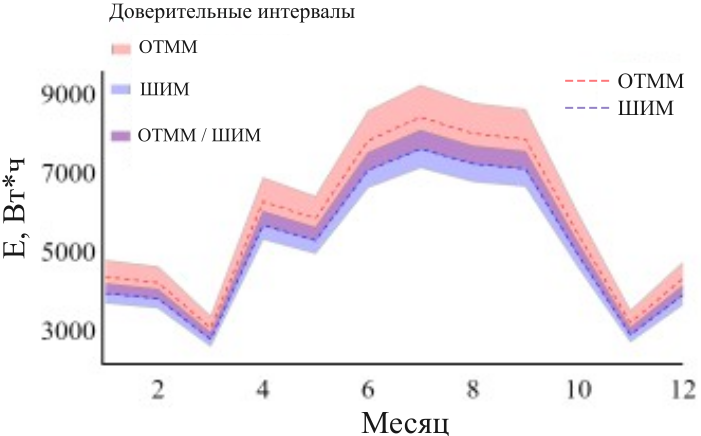
\includegraphics[width=\textwidth]{media/ict/image1}
        \caption*{а)}
    \end{subfigure}
    \hfill
    \begin{subfigure}[b]{0.45\textwidth}
        \centering
        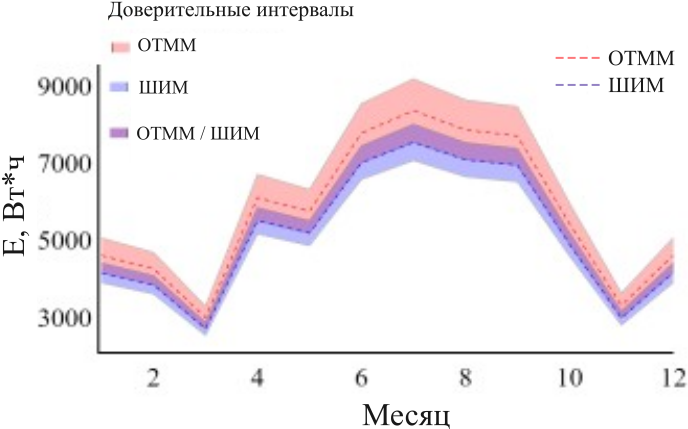
\includegraphics[width=\textwidth]{media/ict/image2}
        \caption*{б)}
    \end{subfigure}

    \par\bigskip

    \begin{subfigure}[b]{0.45\textwidth}
        \centering
        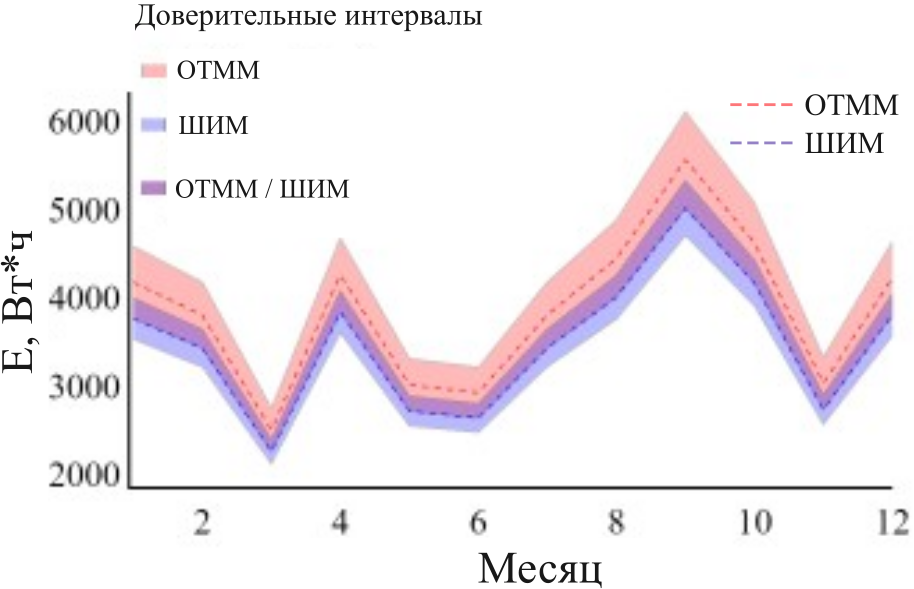
\includegraphics[width=\textwidth]{media/ict/image3}
        \caption*{в)}
    \end{subfigure}
    \caption*{Рис.1 - Диаграммы с ошибками выходной мощности, выработанной каждой фотоэлектрической системой за 1 год: одноосный солнечный трекер (а), двухосный солнечный трекер (б), фиксированная фотоэлектрическая система (в)}
\end{figure}

\begin{multicols}{2}
Как видно из графиков на рисунке 1, выходная мощность систем с одноосным
и двухосным трекерами имеет схожую форму, однако одноосный трекер
генерирует меньше энергии. График для фиксированной фотоэлектрической
установки значительно отличается от первых двух как по форме, так и по
величине мощности. При этом наблюдается область пересечения
доверительных интервалов выходной мощности для систем с контроллерами
ОТММ и ШИМ. Минимальная мощность фиксированной системы составляет 2,6
кВт·ч, а для одноосного и двухосного трекеров она почти одинакова ---
3,8 кВт·ч.

Входная мощность преобразуется с использованием контроллеров ОТММ и ШИМ
для каждой из фотоэлектрических систем, как описано выше. При анализе
системы предполагалось, что средняя выходная мощность при использовании
PWM-контроллера ниже, чем у ОТММ. Однако было выявлено значительное
отклонение в распределении данных для ШИМ, что существенно влияет на его
эффективность. Это можно объяснить более высокой скоростью принятия
решений, присущей контроллеру ОТММ.

Для оценки эффективности работы рассматриваемых контроллеров в сочетании
с различными фотоэлектрическими системами был проведен анализ с
применением двух методов: критерия Стьюдента и критерия
Колмогорова-Смирнова. Критерий Стьюдента представляет собой метод
проверки статистических гипотез, предназначенный для определения
значимости различий между двумя группами данных. В рамках данного
анализа гипотеза \(H_{a}\) заключалась в том, что существует разница в
эффективности работы контроллеров в каждой из рассматриваемых
фотоэлектрических систем. Иными словами, эффективность ОТММ отличается
от эффективности ШИМ. Если гипотеза верна, то выходная мощность одной и
той же системы с разными контроллерами отличается (p\textgreater α), в
противном случае --- идентична (p\textless α). Уровень значимости был
установлен как α = 0.05.

\begin{equation}
H_{a} = \overline{{Eff}_{\text{ОТММ}}}\  \neq \ \overline{{Eff}_{\text{ШИМ}}}
\end{equation}

\begin{equation}
\overline{Eff} = \frac{\sum_{}^{}{Eff}_{i}}{n}
\end{equation}

\begin{equation}
Sd = \ \sqrt{\frac{\sum_{}^{}{({Eff}_{i} - \overline{Eff})}^{2}}{n - 1}}
\end{equation}

\begin{equation}
m_{r} = \ \frac{Sd}{\sqrt{n}}
\end{equation}

\begin{equation}
t = \ \frac{{Eff}_{\text{MPPT}} - {Eff}_{\text{PWM}}\ }{\sqrt{{m_{\text{rотмм}}}^{2} + \ {m_{\text{rшим}}}^{2}}}
\end{equation}

где \(\underline{Eff}\) -- среднее значение показателей эффективности
контроллера, Sd -- стандартное отклонение, \(m_{r}\) -- ошибка
репрезентативности.

Критерий Колмогорова-Смирнова, в свою очередь, является
непараметрическим методом для проверки гипотезы о совпадении
распределений двух выборок. Он широко используется для оценки
соответствия эмпирических данных теоретическому распределению или для
сравнения двух эмпирических распределений. В нашем исследовании этот
тест был использован для дополнительной проверки различий между
контроллерами в каждой фотоэлектрической системе.

Критерий Колмогорова-Смирнова определяется следующим образом:

\begin{equation}
K_{n} = \sqrt{n}*\sup_{x}\left| F_{0}(x) - \widehat{F_{n}}(x) \right|
\end{equation}

Различие между методами t-критерия Стьюдента и критерия
Колмогорова-Смирнова связано с типами информации, которую они
обрабатывают. t-критерий Стьюдента предполагает нормальное и взаимно
независимое распределение данных, в то время как критерий
Колмогорова-Смирнова применяется в случае ненормального распределения
данных. В рамках данного исследования оба метода были использованы для
более полного анализа и проверки гипотезы, что позволило получить более
надежные результаты.

Так как значения выходной мощности сильно зависят от эффективности
контроллеров, были определены максимальные и минимальные пределы
эффективности, как показано на рисунке 1. Для применения статистического
анализа значения эффективности задавались случайным образом в пределах
соответствующего диапазона. Для повышения точности статистического
анализа вычисления повторялись 5000 раз. Результаты анализа каждой
фотоэлектрической системы, работающей с контроллерами ОТММ и ШИМ, были
получены с использованием методов теста Колмогорова-Смирнова и
т-критерия. Для проверки вышеупомянутой гипотезы p-значение должно быть
меньше α=0,05. Из результатов т-критерия, представленных на рисунке 2,
видно, что для одноосного и двухосного трекера p-значение значительно
меньше 0,05 при 5000 повторениях. Следовательно, мы принимаем гипотезу
\(H_{a}\) и делаем вывод, что выходная мощность солнечных трекеров при
использовании различных контроллеров существенно различается. В случае
фиксированной фотоэлектрической системы наблюдаются p-значения в
пределах от 0,046 до 0,27. Среднее p-значение для этой выборки
составляет 0,12, что указывает на меньшую вероятность подтверждения
гипотезы по сравнению с солнечными трекерами.

Результаты теста Колмогорова-Смирнова представлены на рисунке 3. Для
одноосного и двухосного трекера p-значение находится на уровне
10\textsuperscript{-32}, что значительно меньше 0,05 при 5000
повторениях. Следовательно, мы также принимаем выдвинутую гипотезу
\(H_{a}\) и делаем вывод, что выходная мощность солнечных трекеров при
использовании различных контроллеров значительно различается. Для
фиксированной фотоэлектрической системы наблюдаются p-значения в
пределах от 0,1 до 0,85. Среднее p-значение для этой выборки составляет
0,4, что указывает на меньшую вероятность подтверждения гипотезы по
сравнению с трекерами.
\end{multicols}

\begin{figure}[H]
    \centering
    \begin{subfigure}[b]{0.45\textwidth}
        \centering
        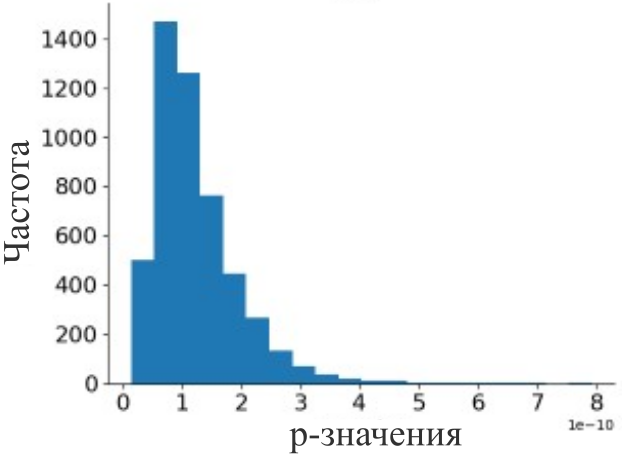
\includegraphics[width=\textwidth]{media/ict/image4}
        \caption*{а)}
    \end{subfigure}
    \hfill
    \begin{subfigure}[b]{0.45\textwidth}
        \centering
        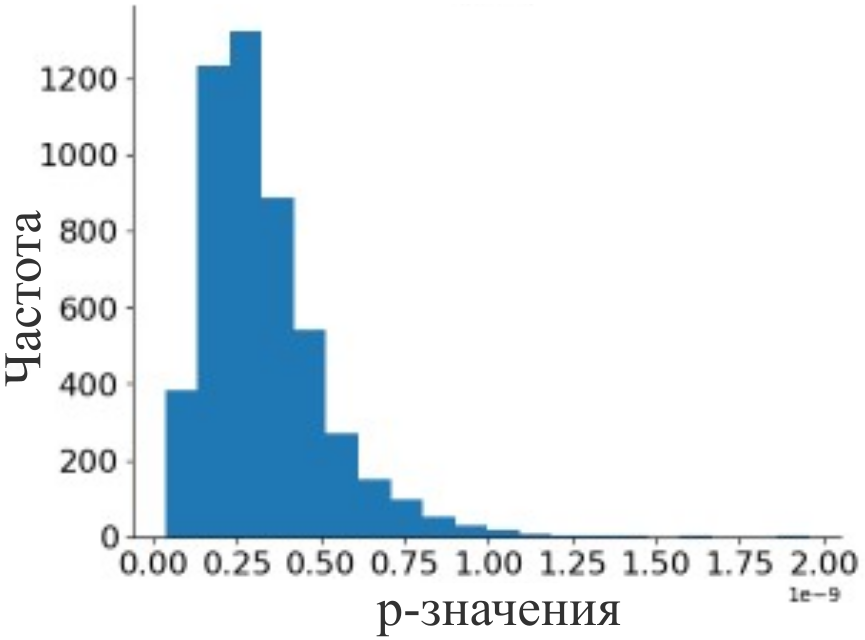
\includegraphics[width=\textwidth]{media/ict/image5}
        \caption*{б)}
    \end{subfigure}

    \par\bigskip

    \begin{subfigure}[b]{0.45\textwidth}
        \centering
        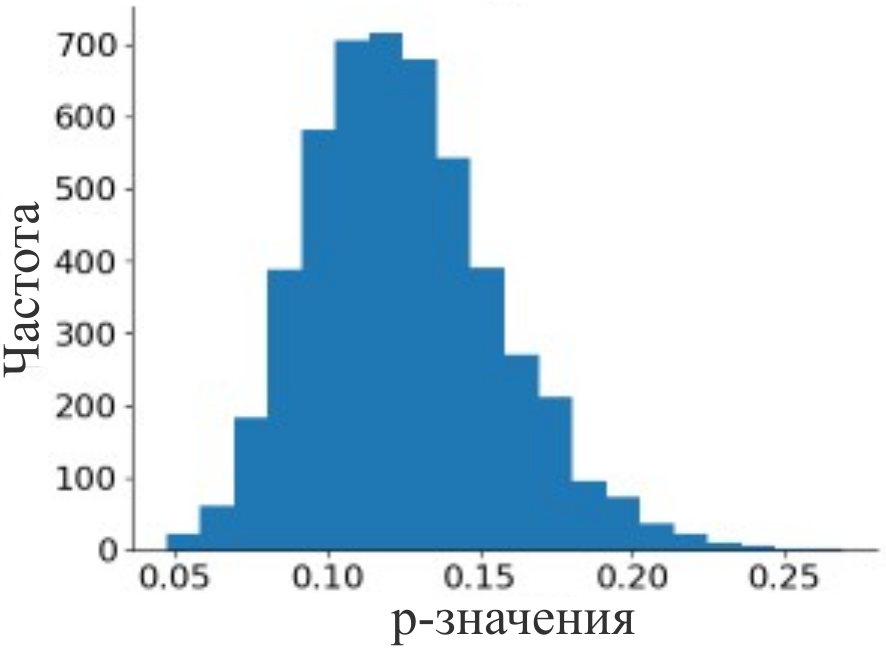
\includegraphics[width=\textwidth]{media/ict/image6}
        \caption*{в)}
    \end{subfigure}
    \caption*{Рис.2 - Результаты т-теста: двухосный солнечный трекер (а), одноосный солнечный трекер (б), фиксированная система (в)}
\end{figure}

\begin{figure}[H]
    \centering
    \begin{subfigure}[b]{0.45\textwidth}
        \centering
        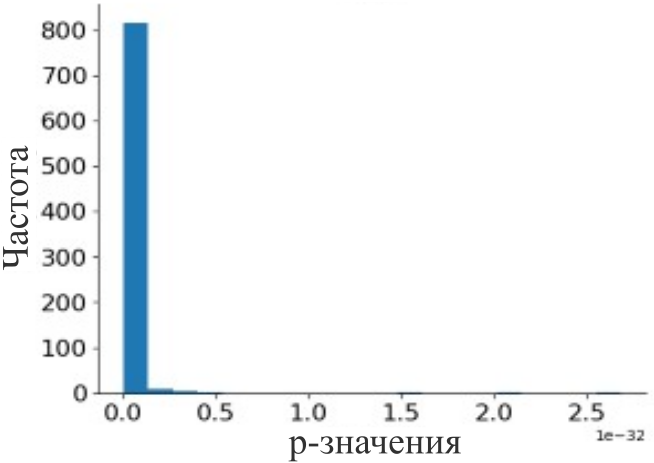
\includegraphics[width=\textwidth]{media/ict/image7}
        \caption*{а)}
    \end{subfigure}
    \hfill
    \begin{subfigure}[b]{0.45\textwidth}
        \centering
        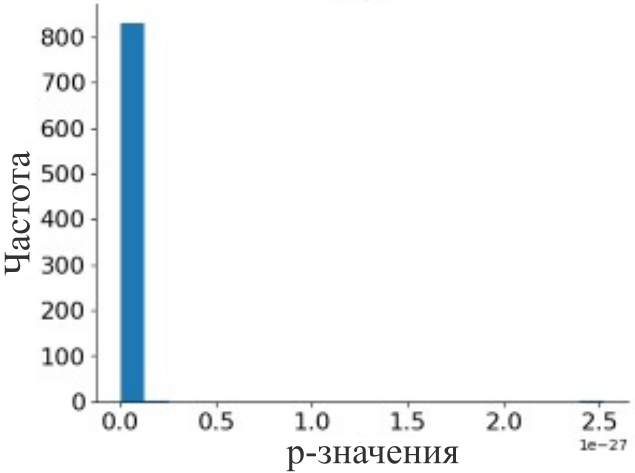
\includegraphics[width=\textwidth]{media/ict/image8}
        \caption*{б)}
    \end{subfigure}

    \par\bigskip

    \begin{subfigure}[b]{0.45\textwidth}
        \centering
        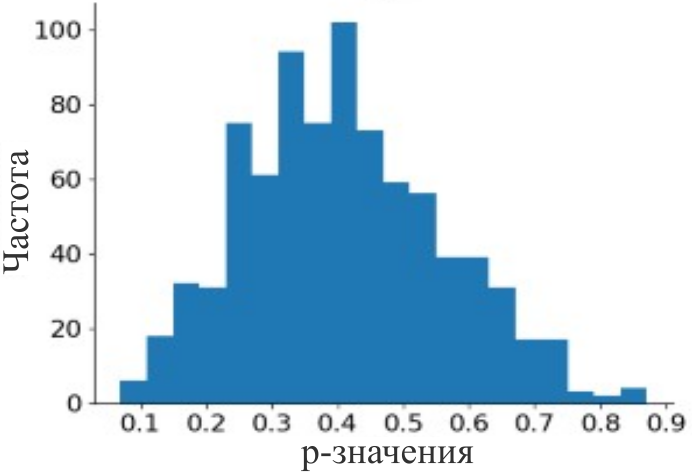
\includegraphics[width=\textwidth]{media/ict/image9}
        \caption*{в)}
    \end{subfigure}
    \caption*{Рис.3 - Результаты теста Колмогорова-Смирнова: двухосный солнечный трекер (а), одноосный солнечный трекер (б), фиксированная система (в)}
\end{figure}

\begin{multicols}{2}
Таким образом, проведенный статистический анализ с использованием
т-критерия Стьюдента и теста Колмогорова-Смирнова позволяет сделать
одинаковый вывод: для фиксированных фотоэлектрических систем
использование контроллеров ОТММ или ШИМ не имеет статистически значимого
влияния.

{\bfseries Результаты и обсуждения.} Цель исследования заключалась в
сравнении эффективности разработанного контроллера зарядки аккумуляторов
с ОТММ и контроллера зарядки аккумуляторов с ШИМ для различных типов
солнечных трекеров в разных погодных условиях. Рисунок 4 показывает
исследуемую экспериментальную установку. На схеме: (1) фиксированная
фотоэлектрическая установка, (2) двухосный солнечный трекер, (3)
одноосный солнечный трекер, (4) электронный блок управления и
аккумуляторы, подключенные к выходу контроллеров зарядки аккумуляторов в
качестве нагрузки, (5) контроллеры ОТММ и ШИМ.

Экспериментальные работы проводились в ясную и частично облачную погоду.
На рисунке 5 представлены графики выходной мощности фиксированной
солнечной панели, одноосного и двухосного трекеров при использовании
контроллера ОТММ. Средняя выходная мощность одноосного трекера с
контроллером ОТММ на 12,8\% и 12,5\% выше, чем у фиксированной системы с
аналогичным контроллером. Выходная мощность двухосного трекера с
контроллером ОТММ на 15\% и 13,4\% выше, чем у фиксированной системы с
тем же контроллером.
\end{multicols}

\begin{figure}[H]
	\centering
	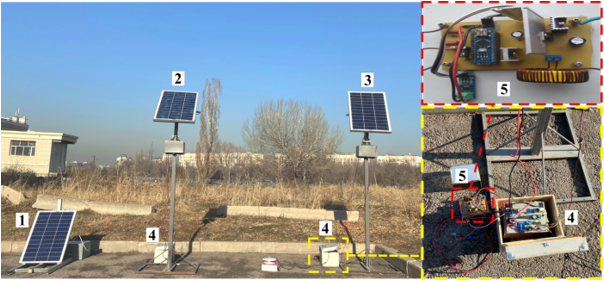
\includegraphics[width=0.8\textwidth]{media/ict/image10}
	\caption*{Рис.4 - Экспериментальная установка}
\end{figure}

\begin{figure}[H]
    \centering
    \begin{subfigure}[b]{0.45\textwidth}
        \centering
        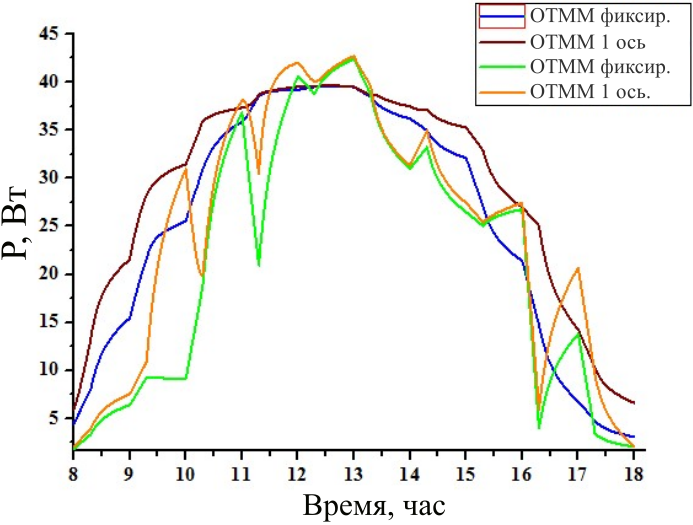
\includegraphics[width=\textwidth]{media/ict/image11}
        \caption*{а)}
    \end{subfigure}
    \hfill
    \begin{subfigure}[b]{0.45\textwidth}
        \centering
        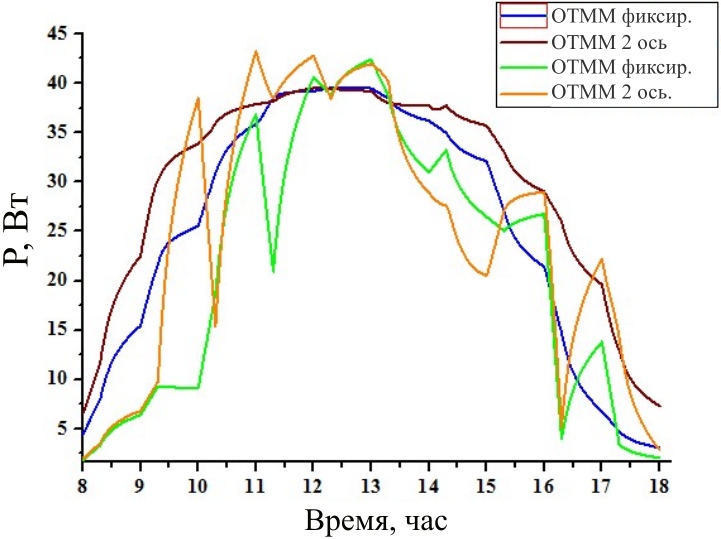
\includegraphics[width=\textwidth]{media/ict/image12}
        \caption*{б)}
    \end{subfigure}
    \caption*{Рис.5 - Сравнение выходной мощности фиксированной солнечной панели с одноосным трекером (а) и двухосным трекером (б) с контроллерами ОТММ}
\end{figure}

\begin{multicols}{2}
Рисунок 6 показывает графики выходной мощности фиксированных панелей,
одноосных и двухосных солнечных трекеров с контроллерами ОТММ и ШИМ.
Эффективность одноосного трекера с контроллером ОТММ на 9,4\% и 10,9\%
выше, чем у системы с контроллером ШИМ. Двухосный солнечный трекер с
контроллером ОТММ преобразует мощность на 10,3\% и 14,2\% эффективнее,
чем с контроллером ШИМ. Фиксированная установка с контроллером ОТММ на
9,5\% и 16,5\% более эффективна, чем фиксированная фотоэлектрическая
установка с контроллером ШИМ.

Максимальная эффективность преобразования мощности соответствует
контроллеру ОТММ с показателем 96\%, в то время как максимальная
эффективность преобразования мощности для контроллера ШИМ достигает
90\%. В то же время минимальный показатель эффективности преобразования
энергии для ОТММ составляет 80\%, а для контроллера ШИМ этот показатель
снижается до 70\%. Эффективность преобразования мощности каждым
контроллером в каждой фотоэлектрической системе показывает различные
результаты.
\end{multicols}

\begin{figure}[H]
    \centering
    \begin{subfigure}[b]{0.45\textwidth}
        \centering
        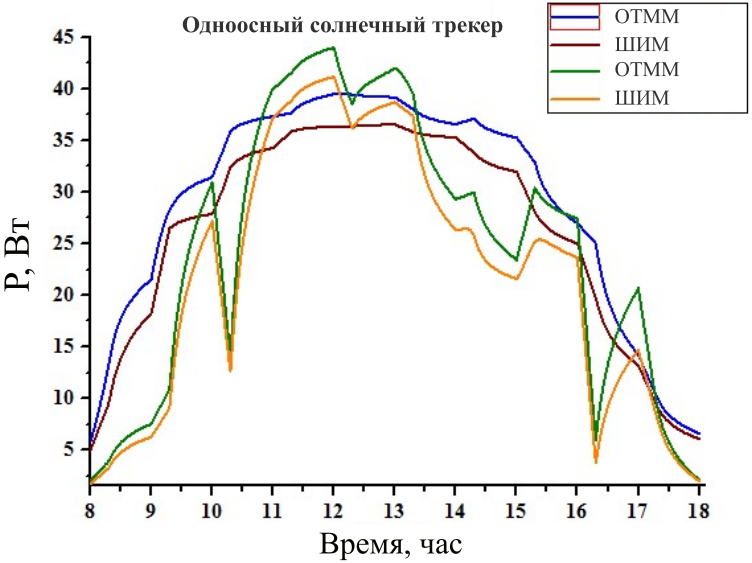
\includegraphics[width=\textwidth]{media/ict/image13}
        \caption*{а)}
    \end{subfigure}
    \hfill
    \begin{subfigure}[b]{0.45\textwidth}
        \centering
        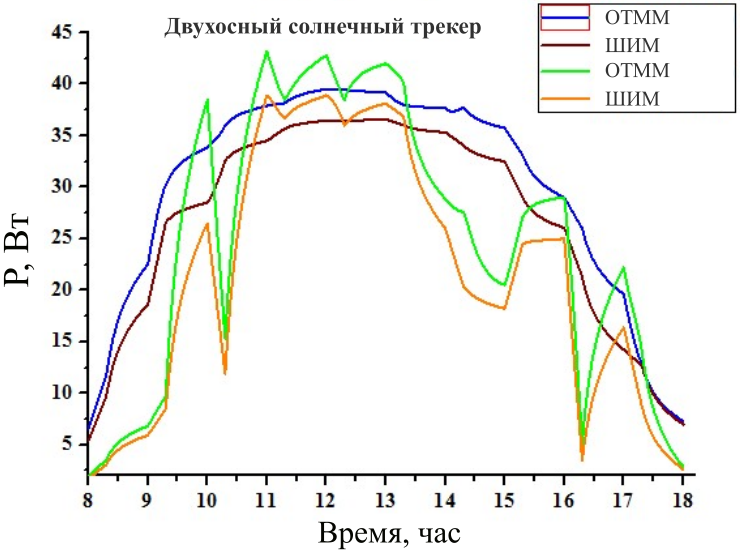
\includegraphics[width=\textwidth]{media/ict/image14}
        \caption*{б)}
    \end{subfigure}

    \par\bigskip

    \begin{subfigure}[b]{0.45\textwidth}
        \centering
        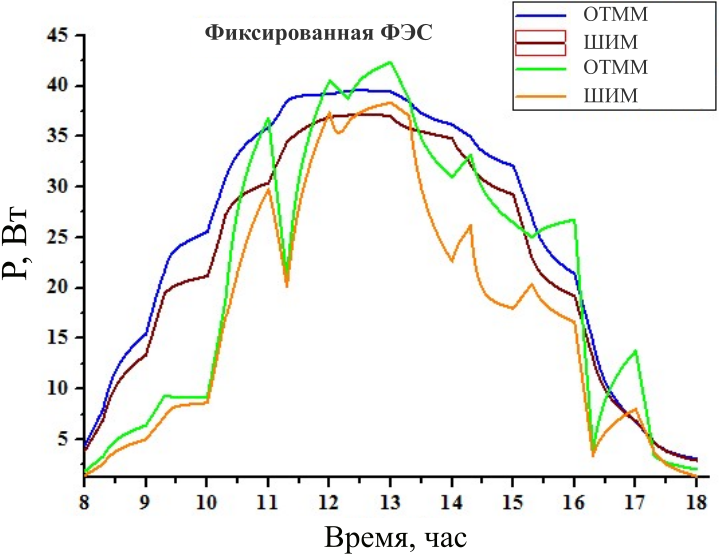
\includegraphics[width=\textwidth]{media/ict/image15}
        \caption*{в)}
    \end{subfigure}
    \caption*{Рис.6 - Графики выходной мощности одноосных (а) и двухосных (б) солнечных трекеров, а также фиксированной системы (в) с контроллерами ОТММ и ШИМ}
\end{figure}


\begin{multicols}{2}
В таблице 1 приведены сравнительные результаты анализа работы
контроллеров ШИМ и ОТММ в сравнении с использованием фиксированной
солнечной панели, одноосного и двухсосного солнечных трекеров с
применением методов т-критерия Стьюдента и теста Колмогорова-Смирнова, а
также соответствующие значения вероятности.
\end{multicols}

\tcap{Таблица 1 - Результаты тестирования статистических гипотез.}
\begin{longtblr}[
  label = none,
  entry = none,
]{
  width = \linewidth,
  colspec = {Q[94]Q[81]Q[94]Q[94]Q[81]Q[94]Q[94]Q[94]Q[202]},
  cells = {c},
  cell{2}{1} = {c=8}{0.726\linewidth},
  cell{3}{5} = {r=2}{},
  cell{3}{6} = {r=2}{},
  cell{3}{7} = {r=2}{},
  cell{3}{8} = {r=2}{},
  cell{3}{9} = {r=2}{},
  cell{5}{1} = {c=8}{0.726\linewidth},
  cell{6}{5} = {r=2}{},
  cell{6}{6} = {r=2}{},
  cell{6}{7} = {r=2}{},
  cell{6}{8} = {r=2}{},
  cell{6}{9} = {r=2}{},
  cell{8}{1} = {c=8}{0.726\linewidth},
  cell{9}{5} = {r=2}{},
  cell{9}{6} = {r=2}{},
  cell{9}{7} = {r=2}{},
  cell{9}{8} = {r=2}{},
  cell{9}{9} = {r=2}{},
  vlines,
  hline{1-3,5-6,8-9,11} = {-}{},
  hline{4,7,10} = {1-4}{},
}
& \(\underline{Eff}\) & \(\sigma\) & \(m_{r}\)        & т     & p      & КС     & p      & Достоверность \\
Фиксированная ФЭ система   &       &        &        &       &        &        &        &               \\
ШИМ                        & 87.9  & 4.022  & 0.8776 & 0.935 & 0.20   & 0.3333 & 0.1963 & 60\%          \\
ОТММ                       & 89.14 & 4.556  & 0.9942 &       &        &        &        &               \\
Одноосный солнечный трекер &       &        &        &       &        &        &        &               \\
ШИМ                        & 86.24 & 4.9398 & 1.0779 & 2.203 & 0.01   & 0.4285 & 0.0410 & 90\%          \\
ОТММ                       & 89.15 & 3.4990 & 0.7635 &       &        &        &        &               \\
Двухосный солнечный трекер &       &        &        &       &        &        &        &               \\
ШИМ                        & 86.17 & 4.9917 & 1.0892 & 2.087 & 0.0025 & 0.4761 & 0.0159 & 95\%          \\
ОТММ                       & 89.06 & 3.9194 & 0.8552 &       &        &        &        &               
\end{longtblr}

\begin{multicols}{2}
Результаты статистического анализа экспериментальных данных,
представленные в таблице 1, показывают, что для фиксированной системы
p-значение больше 0,05 как для т-теста, так и для теста
Колмогорова-Смирнова, что указывает на неверность гипотезы \(H_{a}\) для
фиксированной системы. В то время как для одноосного и двухосного
солнечных трекеров в обоих тестах p-значения меньше 0,05, что позволяет
заключить, что гипотеза \(H_{a}\) верна для этих солнечных
энергетических систем.

{\bfseries Выводы.} В данной работе была оценена целесообразность
использования контроллеров ОТММ и ШИМ для солнечных энергетических
систем. Было выдвинуто предположение, что эффективность ОТММ не равна
эффективности ШИМ, что было проверено с помощью статистических методов:
т-теста Стьюдента и теста Колмогорова-Смирнова. Статистические тесты
проводились на оценочных выходах солнечных панелей, использующих
одноосный, двухосный солнечные трекеры и фиксированную систему в течение
года. Расчеты проводились для контроллеров ОТММ и ШИМ при различных
значениях эффективности. Статистические тесты были выполнены на основе
данных экспериментальных исследований. Результаты тестов как для
расчетных данных, так и для экспериментальных позволяют сделать
следующий вывод: выходная мощность фотоэлектрической системы при
использовании одноосный и двухосный солнечные трекеры сильно зависит от
типа контроллера, в то время как при использовании фиксированной системы
зависимость от типа контроллера минимальна. Таким образом, в
долгосрочной перспективе для фиксированных солнечных установок имеет
смысл устанавливать контроллеры ШИМ для снижения финансовых затрат,
тогда как для солнечных трекеров необходимо использовать контроллеры
ОТММ для максимизации выходной мощности.

{\bfseries Финансирование.} Работа выполнена при поддержке
исследовательского проекта AP23487428 Комитета науки Министерства науки
и высшего образования Республики Казахстан и выполнена в Казахском
Национальном Университете имени аль-Фараби, что с благодарностью
признано авторами.
\end{multicols}

\begin{center}
{\bfseries Литература}
\end{center}

\begin{references}
1. Maka A. O. M., Alabid J. M. Solar energy technology and its roles in
sustainable development //Clean Energy. -- 2022. -- Т.6. -- №.3. --
С.476-483. \href{https://doi.org/10.1093/ce/zkac023}{DOI 10.1093/ce/zkac023}

2. Rajesh T. et al. Design and implementation of an automatic solar
tracking system for a monocrystalline silicon material panel using
MPPT algorithm //Materials Today: Proceedings. -- 2021. -- Т.45. --
С.1783-1789. \href{https://doi.org/10.1016/j.matpr.2020.08.635}{DOI 10.1016/j.matpr.2020.08.635}

3. Rizzo S. A., Scelba G. A hybrid global MPPT searching method for fast
variable shading conditions //Journal of Cleaner Production. -- 2021.
-- Т.298. -- С.126775. \href{https://doi.org/10.1016/j.jclepro.2021.126775}{DOI 10.1016/j.jclepro.2021.126775}

4. Bhukya L., Kedika N. R., Salkuti S. R. Enhanced maximum power point
techniques for solar photovoltaic system under uniform insolation and
partial shading conditions: a review //Algorithms. -- 2022. -- Т.15.
-- №.10. -- С.365. \href{https://doi.org/10.3390/a15100365}{DOI 10.3390/a15100365}

5. Ibrahim N. F. et al. A new adaptive MPPT technique using an improved
INC algorithm supported by fuzzy self-tuning controller for a
grid-linked photovoltaic system //Plos one. -- 2023. -- Т.18. -- №.
61. -- С. e0293613. \href{https://doi.org/10.1371/journal.pone.0293613}{DOI 10.1371/journal.pone.0293613}

6. Bouguerra K., Latreche S., Khemliche M. Comparative Study betwenn
P\&O, IncCond and MSC \\algorithms for MPPT Control of PV systeme
//2023 International Conference on Electrical Engineering and Advanced
Technology (ICEEAT). -- IEEE, 2023. -- Т.1. -- С.1-6.\\
DOI 10.1109/ICEEAT60471.2023.10425855

7. Şenpinar A., Cebeci M. Evaluation of power output for fixed and
two-axis tracking PVarrays //Applied Energy. -- 2012. -- Т.92. -- С.
677-685.
\href{https://doi.org/10.1016/j.apenergy.2011.07.043}{DOI 10.1016/j.apenergy.2011.07.043}

8. Abdulkadir M., Samosir A. S., Yatim A. H. M. Modelling and simulation
of maximum power point tracking of photovoltaic system in Simulink
model //2012 IEEE International Conference on Power and Energy
(PECon). -- IEEE, 2012. -- С.325-330.10.1109/PECon.2012.6450231

9. Mohapatra A. et al. A review on MPPT techniques of PV system under
partial shading condition //Renewable and Sustainable Energy Reviews.
-- 2017. -- Т.80. -- С.854-867.
\href{https://doi.org/10.1016/j.rser.2017.05.083}{DOI \\10.1016/j.rser.2017.05.083}

10. Lazaroiu G. C. et al. Comparative analysis of fixed and sun
tracking low power PV systems considering energy consumption //Energy
Conversion and Management. -- 2015. -- Т.92. -- С.143-148. DOI \\10.1016/j.enconman.2014.12.046

11. \href{https://doi.org/10.1016/j.enconman.2014.12.046\%20}{DOI 10.1016/j.enconman.2014.12.046\%20}
Pulido-Mancebo J. S. et al. Spatial distribution model of solar
radiation for agrivoltaic land use in fixed PV plants //Agronomy. --
2022. -- Т.12. -- №.11. -- С.2799.
\href{https://doi.org/10.3390/agronomy12112799}{DOI 10.3390/agronomy12112799}

12. MacFarland T. W. et al. Student's t-test for independent samples
//Using R for Biostatistics. -- 2021. -- С.141-240.
\href{https://doi.org/10.1007/978-3-030-62404-0_3}{DOI 10.1007/978-3-030-62404-0\_3}

13. Zhang G. et al. Fast and robust spectrum sensing via
Kolmogorov-Smirnov test //IEEE Transactions on Communications. --
2010. -- Т.58. -- №.12. -- С.3410-3416.
DOI 10.1109/TCOMM.2010.11.090209
\end{references}

\begin{authorinfo}
\hspace{1em}\emph{{\bfseries Сведения об авторах}}

Құттыбай Н.Б. -и.о. доцент, PhD, Казахский Национальный Университет
им. аль-Фараби, Алматы, Казахстан, e-mail: \\Nurjigit.10.93@gmail.com;

Байболов Олжас Бауыржанович, магистрант, 1 курс, Казахский
Национальный Университет имени аль-Фараби, Алматы, 050038, Республика
Казахстан, e-mail: baibolov\_olzhas2@kaznu.kz.

\hspace{1em}\emph{{\bfseries Information about the authors}}

Kuttybay N.- acting associate professor, PhD, Kazakh National
University named after аl-Farabi, Almaty, Kazakhstan, e-mail:
Nurjigit.10.93@gmail.com;

Baibolov O.- Master's student, 1st year, Al-Farabi Kazakh National
University, Almaty, Kazakhstan, e-mail: \\baibolov\_olzhas2@kaznu.kz.
\end{authorinfo}
